\documentclass{article}


\usepackage{arxiv}

\usepackage[utf8]{inputenc} % allow utf-8 input
\usepackage[T1]{fontenc}    % use 8-bit T1 fonts
\usepackage{hyperref}       % hyperlinks
\usepackage{url}            % simple URL typesetting
\usepackage{booktabs}       % professional-quality tables
\usepackage{amsfonts}       % blackboard math symbols
\usepackage{nicefrac}       % compact symbols for 1/2, etc.
\usepackage{microtype}      % microtypography
\usepackage{lipsum}
\usepackage{listings}
\usepackage{color}
\usepackage{graphicx}

\definecolor{dkgreen}{rgb}{0,0.6,0}
\definecolor{gray}{rgb}{0.5,0.5,0.5}
\definecolor{mauve}{rgb}{0.58,0,0.82}
\setcounter{page}{5}
\title{A Tracking and Trading Tool for High-Voltage Transmission}


\lstset{frame=tb,
  language=PHP,
  aboveskip=3mm,
  belowskip=3mm,
  showstringspaces=false,
  columns=flexible,
  basicstyle={\small\ttfamily},
  numbers=none,
  numberstyle=\tiny\color{gray},
  keywordstyle=\color{blue},
  commentstyle=\color{dkgreen},
  stringstyle=\color{mauve},
  breaklines=true,
  breakatwhitespace=true,
  tabsize=3
}


\author{
  Jane Almeida\\%\thanks{Use footnote for providing further
    %information about author (webpage, alternative
    %address)---\emph{not} for acknowledging funding agencies.} \\
  Economics Major, Computer Science and Environmental Studies Minor\\
  Lewis \& Clark College\\
  Portland, OR 97219 \\
  \texttt{janealmeida@lclark.edu} \\
  %% examples of more authors
   %\And
 %Elias D.~Striatum \\
  %Department of Electrical Engineering\\
  %Mount-Sheikh University\\
  %Santa Narimana, Levand \\
  %\texttt{stariate@ee.mount-sheikh.edu} \\
  %% \AND
  %% Coauthor \\
  %% Affiliation \\
  %% Address \\a
  %% \texttt{email} \\
  %% \And
  %% Coauthor \\
  %% Affiliation \\
  %% Address \\
  %% \texttt{email} \\
  %% \And
  %% Coauthor \\
  %% Affiliation \\
  %% Address \\
  %% \texttt{email} \\
}

\begin{document}
\maketitle

\begin{abstract}
The western United States lacks an organized competitive wholesale energy market. This fractures energy markets across the west. Consequently, it impacts how electricity is traded between utilities and independent power producers. Without an organized wholesale energy market, each electric utility is responsible for maintaining reliability in their footprint as well as their tools used to support energy trading. A fundamental part of energy trading is ensuring the electricity can move across the grid from the seller to the buyer. In order to trade electricity between counter parties, traders must purchases or use their own capacity on high-voltage transmission lines. Therefore, I created a tool that assists the tracking and trading of high-voltage transmission by creating a website that visually displays the capacity of high-voltage transmission. Additionally, the website can update the database pertaining to transmission trades, enabling the traders to document transmission trades.
\end{abstract}


% keywords can be removed
\keywords{Energy Trading \and High-Voltage Transmission Management \and High-Voltage Transmission Trading \and High-Voltage Transmission Database \and User-Friendly Website 
}


\section{Introduction}
The western United States lacks an organized competitive wholesale energy market. This fractures energy markets across the west. Consequently, it impacts how electricity is traded between utilities and independent power producers. Without an organized wholesale energy market, each electric utility is responsible for maintaining reliability in their footprint as well as their tools used to support energy trading. A fundamental part of energy trading is ensuring the electricity can move across the grid from the seller to the buyer. In order to trade electricity between counter parties, traders must purchases or use their own capacity on high-voltage transmission lines. Therefore, I created a tool that assists the tracking and trading of high-voltage transmission by creating a website that visually displays the capacity of high-voltage transmission. Additionally, the website can update the database pertaining to transmission trades, enabling the traders to document transmission trades. 

\section{Why This Tool Is Useful}
\label{sec:headings}
The lack of a regional organized energy market in the west forces utilities to develop their own trading tool. More often than not, there is a disconnect between what the traders need and what tools are developed to meet those needs. Therefore, I created an example of a tool that would help energy traders. This tool has three main functions: 1) assist the transaction of transmission by interacting with a mock transmission database; and 2) create a visual, dynamic, user-friendly transmission tracking website for energy traders.

\section{The Main Components of the Tool: How it Works}
\subsection{Creating the Database}
I first made the mock database in my Google Cloud Account. I then entered the following commands to create my database: 

\begin{verbatim}

sudo mysql

CREATE DATABASE projectdatabase CHARACTER SET utf8 COLLATE utf8_general_ci; 

USE projectdatabase; 

CREATE TABLE Transmission_Numbers (id int primary key auto_increment, transmission_id int, hourending int, amount int);

\end{verbatim}


These four commands above made it possible for me to develop my database \cite{aaa}. Once I entered in the necessary data I then created my website. 

\subsection{Creating the Website}

My website had three files. The first file which displays my website is ‘main.php’. This file is responsible for the structure of my website and calls the necessary functions to display the correct information from the database I created. My second file, ‘mysql.php’ is responsible for connecting to my database to my website. It is also responsible for all of my SQL functions that interact with my database. The final component to my website is the ‘final.css’ file which is responsible for the stylistic parts of my website, such as color, font, and size of specific ids and classes within ‘main.php’. 

\subsection{Connecting My Database to My Website}
Within my ‘mysql.php’ file I connect my database to my website. I accomplish this by the following section of code: 


\begin{lstlisting}

<?php

/*** connection credentials ***/
$servername = "localhost";
$username = "trader";
$password = "pleasegivemeanAjens";
$database = "projectdatabase";
$usertable1 = "Transmission_Numbers";
$usertable2 = "Transmission_Names";
$dbport = 3306;

/***connect to database***/
try {
$db = new PDO("mysql:host=$servername;dbname=$database;charset=utf8;port=$dbport", $username, $password);
}
catch(PDOException $e) {
echo $e->getMessage();
}

/*** functions interacting with my database would be found below, however, they are emitted for this example ***/
?>

\end{lstlisting}

This section of code made it possible for users of my website to update the database, a crucial part of the tool that made it useful. My website can be found here: \href{http://35.230.57.128/final/main.php}{http://35.230.57.128/final/main.php}. 

    \begin{figure}
        \centering
        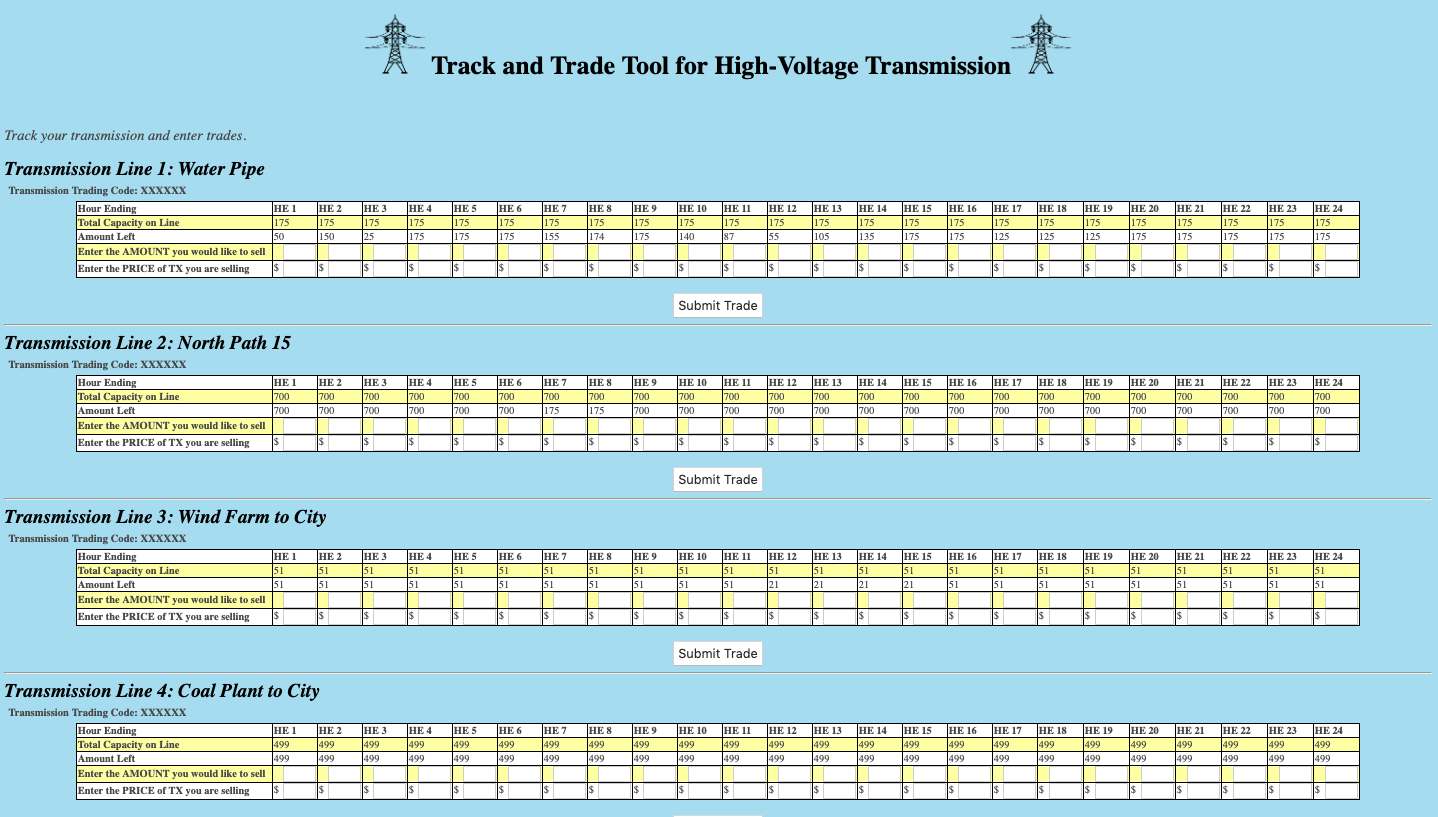
\includegraphics[width=.9\columnwidth]{jane_fig1.png}
        \caption{Screenshot of Final Website}
        \label{fig:my_label}
    \end{figure}



\bibliographystyle{unsrt}  
%\bibliography{references}  %%% Remove comment to use the external .bib file (using bibtex).
%%% and comment out the ``thebibliography'' section.


%%% Comment out this section when you \bibliography{references} is enabled.
\begin{thebibliography}{1}

\bibitem{aaa}
Chapple, M.
\newblock Creating Databases and Tables in SQL
\newblock In {\em Life Wire, 2019}

\end{thebibliography}

\end{document}
